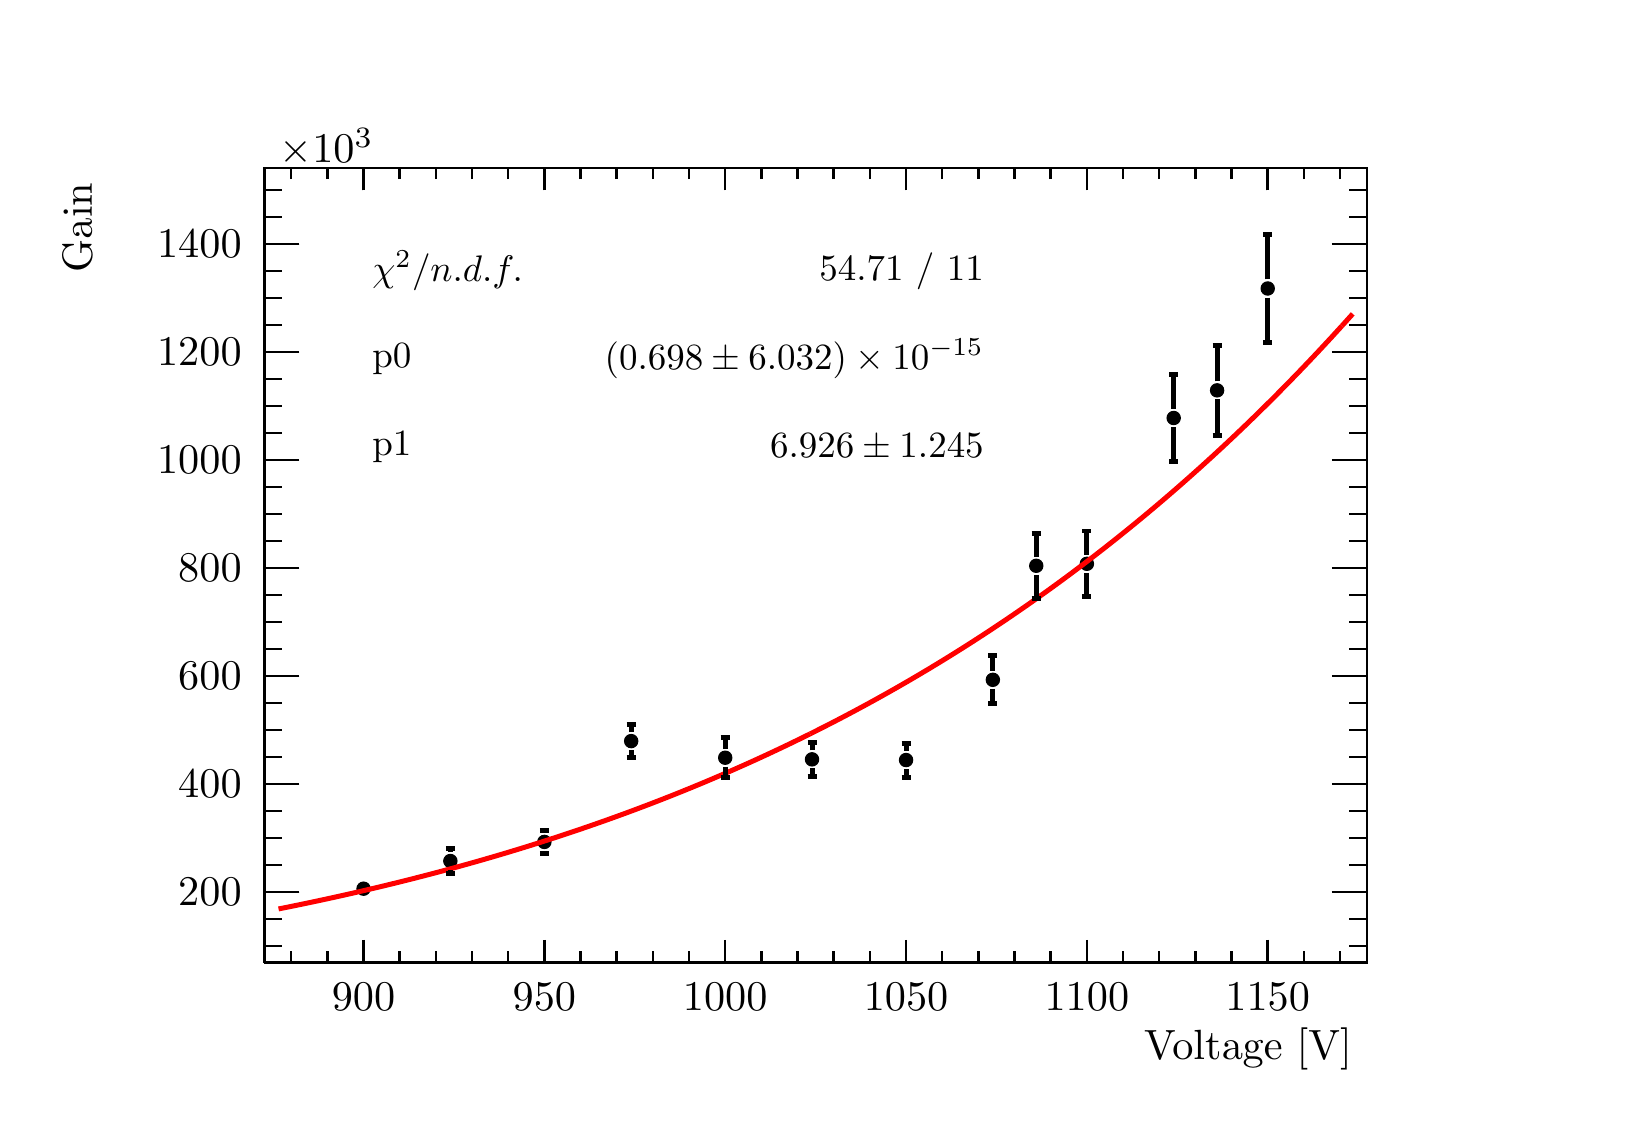
\begin{tikzpicture}
\pgfdeclareplotmark{cross} {
\pgfpathmoveto{\pgfpoint{-0.3\pgfplotmarksize}{\pgfplotmarksize}}
\pgfpathlineto{\pgfpoint{+0.3\pgfplotmarksize}{\pgfplotmarksize}}
\pgfpathlineto{\pgfpoint{+0.3\pgfplotmarksize}{0.3\pgfplotmarksize}}
\pgfpathlineto{\pgfpoint{+1\pgfplotmarksize}{0.3\pgfplotmarksize}}
\pgfpathlineto{\pgfpoint{+1\pgfplotmarksize}{-0.3\pgfplotmarksize}}
\pgfpathlineto{\pgfpoint{+0.3\pgfplotmarksize}{-0.3\pgfplotmarksize}}
\pgfpathlineto{\pgfpoint{+0.3\pgfplotmarksize}{-1.\pgfplotmarksize}}
\pgfpathlineto{\pgfpoint{-0.3\pgfplotmarksize}{-1.\pgfplotmarksize}}
\pgfpathlineto{\pgfpoint{-0.3\pgfplotmarksize}{-0.3\pgfplotmarksize}}
\pgfpathlineto{\pgfpoint{-1.\pgfplotmarksize}{-0.3\pgfplotmarksize}}
\pgfpathlineto{\pgfpoint{-1.\pgfplotmarksize}{0.3\pgfplotmarksize}}
\pgfpathlineto{\pgfpoint{-0.3\pgfplotmarksize}{0.3\pgfplotmarksize}}
\pgfpathclose
\pgfusepathqstroke
}
\pgfdeclareplotmark{cross*} {
\pgfpathmoveto{\pgfpoint{-0.3\pgfplotmarksize}{\pgfplotmarksize}}
\pgfpathlineto{\pgfpoint{+0.3\pgfplotmarksize}{\pgfplotmarksize}}
\pgfpathlineto{\pgfpoint{+0.3\pgfplotmarksize}{0.3\pgfplotmarksize}}
\pgfpathlineto{\pgfpoint{+1\pgfplotmarksize}{0.3\pgfplotmarksize}}
\pgfpathlineto{\pgfpoint{+1\pgfplotmarksize}{-0.3\pgfplotmarksize}}
\pgfpathlineto{\pgfpoint{+0.3\pgfplotmarksize}{-0.3\pgfplotmarksize}}
\pgfpathlineto{\pgfpoint{+0.3\pgfplotmarksize}{-1.\pgfplotmarksize}}
\pgfpathlineto{\pgfpoint{-0.3\pgfplotmarksize}{-1.\pgfplotmarksize}}
\pgfpathlineto{\pgfpoint{-0.3\pgfplotmarksize}{-0.3\pgfplotmarksize}}
\pgfpathlineto{\pgfpoint{-1.\pgfplotmarksize}{-0.3\pgfplotmarksize}}
\pgfpathlineto{\pgfpoint{-1.\pgfplotmarksize}{0.3\pgfplotmarksize}}
\pgfpathlineto{\pgfpoint{-0.3\pgfplotmarksize}{0.3\pgfplotmarksize}}
\pgfpathclose
\pgfusepathqfillstroke
}
\pgfdeclareplotmark{newstar} {
\pgfpathmoveto{\pgfqpoint{0pt}{\pgfplotmarksize}}
\pgfpathlineto{\pgfqpointpolar{44}{0.5\pgfplotmarksize}}
\pgfpathlineto{\pgfqpointpolar{18}{\pgfplotmarksize}}
\pgfpathlineto{\pgfqpointpolar{-20}{0.5\pgfplotmarksize}}
\pgfpathlineto{\pgfqpointpolar{-54}{\pgfplotmarksize}}
\pgfpathlineto{\pgfqpointpolar{-90}{0.5\pgfplotmarksize}}
\pgfpathlineto{\pgfqpointpolar{234}{\pgfplotmarksize}}
\pgfpathlineto{\pgfqpointpolar{198}{0.5\pgfplotmarksize}}
\pgfpathlineto{\pgfqpointpolar{162}{\pgfplotmarksize}}
\pgfpathlineto{\pgfqpointpolar{134}{0.5\pgfplotmarksize}}
\pgfpathclose
\pgfusepathqstroke
}
\pgfdeclareplotmark{newstar*} {
\pgfpathmoveto{\pgfqpoint{0pt}{\pgfplotmarksize}}
\pgfpathlineto{\pgfqpointpolar{44}{0.5\pgfplotmarksize}}
\pgfpathlineto{\pgfqpointpolar{18}{\pgfplotmarksize}}
\pgfpathlineto{\pgfqpointpolar{-20}{0.5\pgfplotmarksize}}
\pgfpathlineto{\pgfqpointpolar{-54}{\pgfplotmarksize}}
\pgfpathlineto{\pgfqpointpolar{-90}{0.5\pgfplotmarksize}}
\pgfpathlineto{\pgfqpointpolar{234}{\pgfplotmarksize}}
\pgfpathlineto{\pgfqpointpolar{198}{0.5\pgfplotmarksize}}
\pgfpathlineto{\pgfqpointpolar{162}{\pgfplotmarksize}}
\pgfpathlineto{\pgfqpointpolar{134}{0.5\pgfplotmarksize}}
\pgfpathclose
\pgfusepathqfillstroke
}
\definecolor{c}{rgb}{1,1,1};
\draw [color=c, fill=c] (0,0) rectangle (20,13.639);
\draw [color=c, fill=c] (3,1.77307) rectangle (17,11.8659);
\definecolor{c}{rgb}{0,0,0};
\draw [c,line width=0.9] (3,1.77307) -- (3,11.8659) -- (17,11.8659) -- (17,1.77307) -- (3,1.77307);
\definecolor{c}{rgb}{1,1,1};
\draw [color=c, fill=c] (3,1.77307) rectangle (17,11.8659);
\definecolor{c}{rgb}{0,0,0};
\draw [c,line width=0.9] (3,1.77307) -- (3,11.8659) -- (17,11.8659) -- (17,1.77307) -- (3,1.77307);
\draw [c,line width=0.9] (3,1.77307) -- (17,1.77307);
\draw [c,line width=0.9] (4.25853,2.05948) -- (4.25853,1.77307);
\draw [c,line width=0.9] (4.71785,1.91628) -- (4.71785,1.77307);
\draw [c,line width=0.9] (5.17717,1.91628) -- (5.17717,1.77307);
\draw [c,line width=0.9] (5.63648,1.91628) -- (5.63648,1.77307);
\draw [c,line width=0.9] (6.0958,1.91628) -- (6.0958,1.77307);
\draw [c,line width=0.9] (6.55512,2.05948) -- (6.55512,1.77307);
\draw [c,line width=0.9] (7.01444,1.91628) -- (7.01444,1.77307);
\draw [c,line width=0.9] (7.47375,1.91628) -- (7.47375,1.77307);
\draw [c,line width=0.9] (7.93307,1.91628) -- (7.93307,1.77307);
\draw [c,line width=0.9] (8.39239,1.91628) -- (8.39239,1.77307);
\draw [c,line width=0.9] (8.85171,2.05948) -- (8.85171,1.77307);
\draw [c,line width=0.9] (9.31102,1.91628) -- (9.31102,1.77307);
\draw [c,line width=0.9] (9.77034,1.91628) -- (9.77034,1.77307);
\draw [c,line width=0.9] (10.2297,1.91628) -- (10.2297,1.77307);
\draw [c,line width=0.9] (10.689,1.91628) -- (10.689,1.77307);
\draw [c,line width=0.9] (11.1483,2.05948) -- (11.1483,1.77307);
\draw [c,line width=0.9] (11.6076,1.91628) -- (11.6076,1.77307);
\draw [c,line width=0.9] (12.0669,1.91628) -- (12.0669,1.77307);
\draw [c,line width=0.9] (12.5262,1.91628) -- (12.5262,1.77307);
\draw [c,line width=0.9] (12.9856,1.91628) -- (12.9856,1.77307);
\draw [c,line width=0.9] (13.4449,2.05948) -- (13.4449,1.77307);
\draw [c,line width=0.9] (13.9042,1.91628) -- (13.9042,1.77307);
\draw [c,line width=0.9] (14.3635,1.91628) -- (14.3635,1.77307);
\draw [c,line width=0.9] (14.8228,1.91628) -- (14.8228,1.77307);
\draw [c,line width=0.9] (15.2822,1.91628) -- (15.2822,1.77307);
\draw [c,line width=0.9] (15.7415,2.05948) -- (15.7415,1.77307);
\draw [c,line width=0.9] (4.25853,2.05948) -- (4.25853,1.77307);
\draw [c,line width=0.9] (3.79921,1.91628) -- (3.79921,1.77307);
\draw [c,line width=0.9] (3.3399,1.91628) -- (3.3399,1.77307);
\draw [c,line width=0.9] (15.7415,2.05948) -- (15.7415,1.77307);
\draw [c,line width=0.9] (16.2008,1.91628) -- (16.2008,1.77307);
\draw [c,line width=0.9] (16.6601,1.91628) -- (16.6601,1.77307);
\draw [anchor=base] (4.25853,1.15931) node[scale=1.52731, color=c, rotate=0]{900};
\draw [anchor=base] (6.55512,1.15931) node[scale=1.52731, color=c, rotate=0]{950};
\draw [anchor=base] (8.85171,1.15931) node[scale=1.52731, color=c, rotate=0]{1000};
\draw [anchor=base] (11.1483,1.15931) node[scale=1.52731, color=c, rotate=0]{1050};
\draw [anchor=base] (13.4449,1.15931) node[scale=1.52731, color=c, rotate=0]{1100};
\draw [anchor=base] (15.7415,1.15931) node[scale=1.52731, color=c, rotate=0]{1150};
\draw [anchor= east] (17,0.681948) node[scale=1.52731, color=c, rotate=0]{ Voltage [V]};
\draw [c,line width=0.9] (3,11.8659) -- (17,11.8659);
\draw [c,line width=0.9] (4.25853,11.5795) -- (4.25853,11.8659);
\draw [c,line width=0.9] (4.71785,11.7227) -- (4.71785,11.8659);
\draw [c,line width=0.9] (5.17717,11.7227) -- (5.17717,11.8659);
\draw [c,line width=0.9] (5.63648,11.7227) -- (5.63648,11.8659);
\draw [c,line width=0.9] (6.0958,11.7227) -- (6.0958,11.8659);
\draw [c,line width=0.9] (6.55512,11.5795) -- (6.55512,11.8659);
\draw [c,line width=0.9] (7.01444,11.7227) -- (7.01444,11.8659);
\draw [c,line width=0.9] (7.47375,11.7227) -- (7.47375,11.8659);
\draw [c,line width=0.9] (7.93307,11.7227) -- (7.93307,11.8659);
\draw [c,line width=0.9] (8.39239,11.7227) -- (8.39239,11.8659);
\draw [c,line width=0.9] (8.85171,11.5795) -- (8.85171,11.8659);
\draw [c,line width=0.9] (9.31102,11.7227) -- (9.31102,11.8659);
\draw [c,line width=0.9] (9.77034,11.7227) -- (9.77034,11.8659);
\draw [c,line width=0.9] (10.2297,11.7227) -- (10.2297,11.8659);
\draw [c,line width=0.9] (10.689,11.7227) -- (10.689,11.8659);
\draw [c,line width=0.9] (11.1483,11.5795) -- (11.1483,11.8659);
\draw [c,line width=0.9] (11.6076,11.7227) -- (11.6076,11.8659);
\draw [c,line width=0.9] (12.0669,11.7227) -- (12.0669,11.8659);
\draw [c,line width=0.9] (12.5262,11.7227) -- (12.5262,11.8659);
\draw [c,line width=0.9] (12.9856,11.7227) -- (12.9856,11.8659);
\draw [c,line width=0.9] (13.4449,11.5795) -- (13.4449,11.8659);
\draw [c,line width=0.9] (13.9042,11.7227) -- (13.9042,11.8659);
\draw [c,line width=0.9] (14.3635,11.7227) -- (14.3635,11.8659);
\draw [c,line width=0.9] (14.8228,11.7227) -- (14.8228,11.8659);
\draw [c,line width=0.9] (15.2822,11.7227) -- (15.2822,11.8659);
\draw [c,line width=0.9] (15.7415,11.5795) -- (15.7415,11.8659);
\draw [c,line width=0.9] (4.25853,11.5795) -- (4.25853,11.8659);
\draw [c,line width=0.9] (3.79921,11.7227) -- (3.79921,11.8659);
\draw [c,line width=0.9] (3.3399,11.7227) -- (3.3399,11.8659);
\draw [c,line width=0.9] (15.7415,11.5795) -- (15.7415,11.8659);
\draw [c,line width=0.9] (16.2008,11.7227) -- (16.2008,11.8659);
\draw [c,line width=0.9] (16.6601,11.7227) -- (16.6601,11.8659);
\draw [c,line width=0.9] (3,1.77307) -- (3,11.8659);
\draw [c,line width=0.9] (3.444,2.67094) -- (3,2.67094);
\draw [c,line width=0.9] (3.222,3.01379) -- (3,3.01379);
\draw [c,line width=0.9] (3.222,3.35663) -- (3,3.35663);
\draw [c,line width=0.9] (3.222,3.69948) -- (3,3.69948);
\draw [c,line width=0.9] (3.444,4.04233) -- (3,4.04233);
\draw [c,line width=0.9] (3.222,4.38517) -- (3,4.38517);
\draw [c,line width=0.9] (3.222,4.72802) -- (3,4.72802);
\draw [c,line width=0.9] (3.222,5.07086) -- (3,5.07086);
\draw [c,line width=0.9] (3.444,5.41371) -- (3,5.41371);
\draw [c,line width=0.9] (3.222,5.75656) -- (3,5.75656);
\draw [c,line width=0.9] (3.222,6.0994) -- (3,6.0994);
\draw [c,line width=0.9] (3.222,6.44225) -- (3,6.44225);
\draw [c,line width=0.9] (3.444,6.78509) -- (3,6.78509);
\draw [c,line width=0.9] (3.222,7.12794) -- (3,7.12794);
\draw [c,line width=0.9] (3.222,7.47078) -- (3,7.47078);
\draw [c,line width=0.9] (3.222,7.81363) -- (3,7.81363);
\draw [c,line width=0.9] (3.444,8.15648) -- (3,8.15648);
\draw [c,line width=0.9] (3.222,8.49932) -- (3,8.49932);
\draw [c,line width=0.9] (3.222,8.84217) -- (3,8.84217);
\draw [c,line width=0.9] (3.222,9.18501) -- (3,9.18501);
\draw [c,line width=0.9] (3.444,9.52786) -- (3,9.52786);
\draw [c,line width=0.9] (3.222,9.8707) -- (3,9.8707);
\draw [c,line width=0.9] (3.222,10.2136) -- (3,10.2136);
\draw [c,line width=0.9] (3.222,10.5564) -- (3,10.5564);
\draw [c,line width=0.9] (3.444,10.8992) -- (3,10.8992);
\draw [c,line width=0.9] (3.444,2.67094) -- (3,2.67094);
\draw [c,line width=0.9] (3.222,2.3281) -- (3,2.3281);
\draw [c,line width=0.9] (3.222,1.98525) -- (3,1.98525);
\draw [c,line width=0.9] (3.444,10.8992) -- (3,10.8992);
\draw [c,line width=0.9] (3.222,11.2421) -- (3,11.2421);
\draw [c,line width=0.9] (3.222,11.5849) -- (3,11.5849);
\draw [anchor= east] (2.9,2.67094) node[scale=1.52731, color=c, rotate=0]{200};
\draw [anchor= east] (2.9,4.04233) node[scale=1.52731, color=c, rotate=0]{400};
\draw [anchor= east] (2.9,5.41371) node[scale=1.52731, color=c, rotate=0]{600};
\draw [anchor= east] (2.9,6.78509) node[scale=1.52731, color=c, rotate=0]{800};
\draw [anchor= east] (2.9,8.15648) node[scale=1.52731, color=c, rotate=0]{1000};
\draw [anchor= east] (2.9,9.52786) node[scale=1.52731, color=c, rotate=0]{1200};
\draw [anchor= east] (2.9,10.8992) node[scale=1.52731, color=c, rotate=0]{1400};
\draw [anchor=base west] (3,11.9341) node[scale=1.52731, color=c, rotate=0]{$\times10^{3}$};
\draw [anchor= east] (0.624642,11.8659) node[scale=1.52731, color=c, rotate=90]{ Gain};
\draw [c,line width=0.9] (17,1.77307) -- (17,11.8659);
\draw [c,line width=0.9] (16.556,2.67094) -- (17,2.67094);
\draw [c,line width=0.9] (16.778,3.01379) -- (17,3.01379);
\draw [c,line width=0.9] (16.778,3.35663) -- (17,3.35663);
\draw [c,line width=0.9] (16.778,3.69948) -- (17,3.69948);
\draw [c,line width=0.9] (16.556,4.04233) -- (17,4.04233);
\draw [c,line width=0.9] (16.778,4.38517) -- (17,4.38517);
\draw [c,line width=0.9] (16.778,4.72802) -- (17,4.72802);
\draw [c,line width=0.9] (16.778,5.07086) -- (17,5.07086);
\draw [c,line width=0.9] (16.556,5.41371) -- (17,5.41371);
\draw [c,line width=0.9] (16.778,5.75656) -- (17,5.75656);
\draw [c,line width=0.9] (16.778,6.0994) -- (17,6.0994);
\draw [c,line width=0.9] (16.778,6.44225) -- (17,6.44225);
\draw [c,line width=0.9] (16.556,6.78509) -- (17,6.78509);
\draw [c,line width=0.9] (16.778,7.12794) -- (17,7.12794);
\draw [c,line width=0.9] (16.778,7.47078) -- (17,7.47078);
\draw [c,line width=0.9] (16.778,7.81363) -- (17,7.81363);
\draw [c,line width=0.9] (16.556,8.15648) -- (17,8.15648);
\draw [c,line width=0.9] (16.778,8.49932) -- (17,8.49932);
\draw [c,line width=0.9] (16.778,8.84217) -- (17,8.84217);
\draw [c,line width=0.9] (16.778,9.18501) -- (17,9.18501);
\draw [c,line width=0.9] (16.556,9.52786) -- (17,9.52786);
\draw [c,line width=0.9] (16.778,9.8707) -- (17,9.8707);
\draw [c,line width=0.9] (16.778,10.2136) -- (17,10.2136);
\draw [c,line width=0.9] (16.778,10.5564) -- (17,10.5564);
\draw [c,line width=0.9] (16.556,10.8992) -- (17,10.8992);
\draw [c,line width=0.9] (16.556,2.67094) -- (17,2.67094);
\draw [c,line width=0.9] (16.778,2.3281) -- (17,2.3281);
\draw [c,line width=0.9] (16.778,1.98525) -- (17,1.98525);
\draw [c,line width=0.9] (16.556,10.8992) -- (17,10.8992);
\draw [c,line width=0.9] (16.778,11.2421) -- (17,11.2421);
\draw [c,line width=0.9] (16.778,11.5849) -- (17,11.5849);
\foreach \P in {(4.25853,2.71105), (5.36089,3.06272), (6.55512,3.30505), (7.65748,4.5854), (8.85171,4.37434), (9.95407,4.35366), (11.1483,4.34486), (12.2507,5.36374), (12.8018,6.81202), (13.4449,6.83732), (14.5472,8.68883), (15.0984,9.03984),
 (15.7415,10.3335)}{\draw[mark options={color=c,fill=c},mark size=2.402402pt,mark=*] plot coordinates {\P};}
\definecolor{c}{rgb}{1,0,0};
\draw [c,line width=1.8] (3.17913,2.45386) -- (3.31693,2.4815) -- (3.45472,2.50971) -- (3.59252,2.53849) -- (3.73031,2.56786) -- (3.86811,2.59782) -- (4.00591,2.62838) -- (4.1437,2.65956) -- (4.2815,2.69136) -- (4.41929,2.72379) -- (4.55709,2.75687)
 -- (4.69488,2.7906) -- (4.83268,2.825) -- (4.97047,2.86008) -- (5.10827,2.89584) -- (5.24606,2.93231) -- (5.38386,2.96948) -- (5.52165,3.00738) -- (5.65945,3.04601) -- (5.79724,3.08538) -- (5.93504,3.12551) -- (6.07283,3.16641) -- (6.21063,3.2081)
 -- (6.34843,3.25057) -- (6.48622,3.29385) -- (6.62402,3.33796) -- (6.76181,3.38289) -- (6.89961,3.42867) -- (7.0374,3.4753) -- (7.1752,3.52281) -- (7.31299,3.5712) -- (7.45079,3.62049) -- (7.58858,3.67069) -- (7.72638,3.72182) -- (7.86417,3.77389)
 -- (8.00197,3.82691) -- (8.13976,3.88091) -- (8.27756,3.93588) -- (8.41535,3.99186) -- (8.55315,4.04885) -- (8.69094,4.10687) -- (8.82874,4.16593) -- (8.96654,4.22605) -- (9.10433,4.28725) -- (9.24213,4.34954) -- (9.37992,4.41294) --
 (9.51772,4.47746) -- (9.65551,4.54312) -- (9.79331,4.60994) -- (9.9311,4.67794);
\draw [c,line width=1.8] (9.9311,4.67794) -- (10.0689,4.74712) -- (10.2067,4.81752) -- (10.3445,4.88914) -- (10.4823,4.962) -- (10.6201,5.03613) -- (10.7579,5.11154) -- (10.8957,5.18824) -- (11.0335,5.26627) -- (11.1713,5.34562) -- (11.3091,5.42633)
 -- (11.4469,5.50842) -- (11.5846,5.5919) -- (11.7224,5.67679) -- (11.8602,5.76311) -- (11.998,5.85089) -- (12.1358,5.94014) -- (12.2736,6.03088) -- (12.4114,6.12314) -- (12.5492,6.21693) -- (12.687,6.31228) -- (12.8248,6.4092) -- (12.9626,6.50772)
 -- (13.1004,6.60787) -- (13.2382,6.70966) -- (13.376,6.81311) -- (13.5138,6.91825) -- (13.6516,7.0251) -- (13.7894,7.13369) -- (13.9272,7.24403) -- (14.065,7.35615) -- (14.2028,7.47008) -- (14.3406,7.58584) -- (14.4783,7.70345) -- (14.6161,7.82294)
 -- (14.7539,7.94433) -- (14.8917,8.06765) -- (15.0295,8.19291) -- (15.1673,8.32016) -- (15.3051,8.44942) -- (15.4429,8.5807) -- (15.5807,8.71404) -- (15.7185,8.84947) -- (15.8563,8.98701) -- (15.9941,9.12668) -- (16.1319,9.26852) --
 (16.2697,9.41255) -- (16.4075,9.55881) -- (16.5453,9.70732) -- (16.6831,9.8581);
\draw [c,line width=1.8] (16.6831,9.8581) -- (16.8209,10.0112);
\definecolor{c}{rgb}{1,1,1};
\draw [color=c, fill=c] (3.75358,7.76504) rectangle (12.7507,11.1175);
\definecolor{c}{rgb}{0,0,0};
\draw [anchor= west] (4.20344,10.5587) node[scale=1.3364, color=c, rotate=0]{$\chi^{2} / \text{n.d.f.} $};
\draw [anchor= east] (12.3009,10.5587) node[scale=1.3364, color=c, rotate=0]{ 54.71 / 11};
\draw [anchor= west] (4.20344,9.44126) node[scale=1.3364, color=c, rotate=0]{p0       };
\draw [anchor= east] (12.3009,9.44126) node[scale=1.3364, color=c, rotate=0]{$ \num{6.978d-16} \pm \num{6.032d-15}$};
\draw [anchor= west] (4.20344,8.32378) node[scale=1.3364, color=c, rotate=0]{p1       };
\draw [anchor= east] (12.3009,8.32378) node[scale=1.3364, color=c, rotate=0]{$ 6.926 \pm 1.245$};
\draw [c,line width=1.8] (5.36089,3.17734) -- (5.36089,3.2271);
\draw [c,line width=1.8] (5.30359,3.2271) -- (5.4182,3.2271);
\draw [c,line width=1.8] (5.36089,2.94811) -- (5.36089,2.89834);
\draw [c,line width=1.8] (5.30359,2.89834) -- (5.4182,2.89834);
\draw [c,line width=1.8] (6.55512,3.41967) -- (6.55512,3.44871);
\draw [c,line width=1.8] (6.49781,3.44871) -- (6.61242,3.44871);
\draw [c,line width=1.8] (6.55512,3.19044) -- (6.55512,3.1614);
\draw [c,line width=1.8] (6.49781,3.1614) -- (6.61242,3.1614);
\draw [c,line width=1.8] (7.65748,4.70001) -- (7.65748,4.79579);
\draw [c,line width=1.8] (7.60017,4.79579) -- (7.71479,4.79579);
\draw [c,line width=1.8] (7.65748,4.47078) -- (7.65748,4.375);
\draw [c,line width=1.8] (7.60017,4.375) -- (7.71479,4.375);
\draw [c,line width=1.8] (8.85171,4.48895) -- (8.85171,4.63068);
\draw [c,line width=1.8] (8.7944,4.63068) -- (8.90901,4.63068);
\draw [c,line width=1.8] (8.85171,4.25973) -- (8.85171,4.118);
\draw [c,line width=1.8] (8.7944,4.118) -- (8.90901,4.118);
\draw [c,line width=1.8] (9.95407,4.46827) -- (9.95407,4.57027);
\draw [c,line width=1.8] (9.89676,4.57027) -- (10.0114,4.57027);
\draw [c,line width=1.8] (9.95407,4.23905) -- (9.95407,4.13706);
\draw [c,line width=1.8] (9.89676,4.13706) -- (10.0114,4.13706);
\draw [c,line width=1.8] (11.1483,4.45948) -- (11.1483,4.56081);
\draw [c,line width=1.8] (11.091,4.56081) -- (11.2056,4.56081);
\draw [c,line width=1.8] (11.1483,4.23025) -- (11.1483,4.12891);
\draw [c,line width=1.8] (11.091,4.12891) -- (11.2056,4.12891);
\draw [c,line width=1.8] (12.2507,5.47835) -- (12.2507,5.6703);
\draw [c,line width=1.8] (12.1933,5.6703) -- (12.308,5.6703);
\draw [c,line width=1.8] (12.2507,5.24913) -- (12.2507,5.05718);
\draw [c,line width=1.8] (12.1933,5.05718) -- (12.308,5.05718);
\draw [c,line width=1.8] (12.8018,6.92663) -- (12.8018,7.22262);
\draw [c,line width=1.8] (12.7445,7.22262) -- (12.8591,7.22262);
\draw [c,line width=1.8] (12.8018,6.6974) -- (12.8018,6.40141);
\draw [c,line width=1.8] (12.7445,6.40141) -- (12.8591,6.40141);
\draw [c,line width=1.8] (13.4449,6.95193) -- (13.4449,7.25373);
\draw [c,line width=1.8] (13.3876,7.25373) -- (13.5022,7.25373);
\draw [c,line width=1.8] (13.4449,6.7227) -- (13.4449,6.4209);
\draw [c,line width=1.8] (13.3876,6.4209) -- (13.5022,6.4209);
\draw [c,line width=1.8] (14.5472,8.80345) -- (14.5472,9.24699);
\draw [c,line width=1.8] (14.4899,9.24699) -- (14.6046,9.24699);
\draw [c,line width=1.8] (14.5472,8.57422) -- (14.5472,8.13068);
\draw [c,line width=1.8] (14.4899,8.13068) -- (14.6046,8.13068);
\draw [c,line width=1.8] (15.0984,9.15446) -- (15.0984,9.614);
\draw [c,line width=1.8] (15.0411,9.614) -- (15.1557,9.614);
\draw [c,line width=1.8] (15.0984,8.92523) -- (15.0984,8.46569);
\draw [c,line width=1.8] (15.0411,8.46569) -- (15.1557,8.46569);
\draw [c,line width=1.8] (15.7415,10.4481) -- (15.7415,11.0248);
\draw [c,line width=1.8] (15.6842,11.0248) -- (15.7988,11.0248);
\draw [c,line width=1.8] (15.7415,10.2189) -- (15.7415,9.64217);
\draw [c,line width=1.8] (15.6842,9.64217) -- (15.7988,9.64217);
\definecolor{c}{rgb}{1,1,1};
\draw [color=c, fill=c] (3.75358,7.76504) rectangle (12.7507,11.1175);
\definecolor{c}{rgb}{0,0,0};
\draw [anchor= west] (4.20344,10.5587) node[scale=1.3364, color=c, rotate=0]{$\chi^{2} / \text{n.d.f.} $};
\draw [anchor= east] (12.3009,10.5587) node[scale=1.3364, color=c, rotate=0]{ 54.71 / 11};
\draw [anchor= west] (4.20344,9.44126) node[scale=1.3364, color=c, rotate=0]{p0       };
\draw [anchor= east] (12.3009,9.44126) node[scale=1.3364, color=c, rotate=0]{$ (0.698 \pm 6.032) \times 10^{-15}$};
\draw [anchor= west] (4.20344,8.32378) node[scale=1.3364, color=c, rotate=0]{p1       };
\draw [anchor= east] (12.3009,8.32378) node[scale=1.3364, color=c, rotate=0]{$ 6.926 \pm 1.245$};
\definecolor{c}{rgb}{1,1,1};
\draw [color=c, fill=c] (2,12.8206) rectangle (18,13.5708);
\definecolor{c}{rgb}{0,0,0};
%\draw (10,13.1957) node[scale=1.20912, color=c, rotate=0]{PMT gain with varying voltage (PMT 0446, 1.5V amp., 1.5V offset)};
\end{tikzpicture}
